\section{Results}
\label{sec:results}

In this section we present a comparison of NLO QCD and NLO QCD+EW predictions for three different processes: DY lepton-pair production, top-pair production, and finally Z-boson (lepton-pair) production with non-zero transverse momentum at the LHC.

Our first aim is a technical one, namely to show the validity of the results reconstructed with the \textsc{PineAPPL} grids introduced in section~\ref{sec:pineappl} and to give a measure of accuracy that can be achieved with them.
The second aim is to quantify the size of the EW corrections for the setups defined by the experimental collaborations for the processes given below.

The following processes are either already part of PDF determinations (7 and \SI{8}{\tera\electronvolt}) in refs.~\cite{} or will likely be part of next-generation PDF fits (\SI{13}{\tera\electronvolt}).
We discuss,
\begin{itemize}
\item in section~\ref{sec:atlas-high-mass-dy}, ATLAS high-mass DY lepton-pair production at \SI{7}{\tera\electronvolt} \cite{Aad:2013iua}, measuring $\mathrm{d} \sigma / \mathrm{d} M_{\ell \bar{\ell}}$ for the lepton-pair invariant mass $M_{\ell \bar{\ell}} > \SI{116}{\giga\electronvolt}$,
\item in section~\ref{sec:cms-dy}, CMS DY lepton-pair production at \SI{7}{\tera\electronvolt} \cite{Chatrchyan:2013tia}, measuring $\mathrm{d} \sigma / \mathrm{d} y_{\ell \bar{\ell}}$ for six slices in the range $\SI{20}{\giga\electronvolt} < M_{\ell \bar{\ell}} < \SI{1500}{\giga\electronvolt}$,
\item in section~\ref{sec:atlas-top-pair-production}, ATLAS top-pair production at \SI{8}{\tera\electronvolt} \cite{Aad:2015mbv}, measuring
\begin{itemize}
\item the transverse momentum of the reconstructed top, $\mathrm{d} \sigma / \mathrm{d} p_\mathrm{T}^\mathrm{t}$,
\item its rapidity, $\mathrm{d} \sigma / \mathrm{d} y_\mathrm{t}$,
\item the invariant mass of the reconstructed top pair, $\mathrm{d} \sigma / \mathrm{d} M_{\mathrm{t} \bar{\mathrm{t}}}$, and
\item its rapidity, $\mathrm{d} \sigma / \mathrm{d} M_{\mathrm{t} \bar{\mathrm{t}}}$,
\end{itemize}
\item in section~\ref{sec:cms-transverse-momentum}, CMS transverse momentum of the Z boson at \SI{13}{\tera\electronvolt} \cite{Sirunyan:2019bzr}, measuring $\mathrm{d} \sigma / \mathrm{d} p_\mathrm{Z}$ for $p_\mathrm{Z} > \SI{20}{\giga\electronvolt}$.
\end{itemize}
We used the MC \texttt{mg5\_aMC@NLO}~\cite{} and the PDF set \texttt{NNPDF31\_as\_0118\_luxqed}~\cite{} to generate the predictions.
The chosen PDF set contains a photon PDF calculated from the LUXQED method~\cite{}.
For each process---except top-pair production, which has stable tops in the final state---we use a complex-mass scheme~\cite{} as described in ref.~\cite{}.
The values of the most important parameters are
\begin{equation}
\begin{aligned}
M_\mathrm{W} &= \SI{80}{\giga\electronvolt} \text{,} \quad &
M_\mathrm{Z} &= \SI{90}{\giga\electronvolt} \text{,} \quad &
m_\mathrm{t} &= \SI{170}{\giga\electronvolt} \text{,} \\
\Gamma_\mathrm{W} &= \SI{2}{\giga\electronvolt} \text{,} &
\Gamma_\mathrm{Z} &= \SI{2}{\giga\electronvolt} \text{,} &
G_\mu &= \text{.}
\end{aligned}
\end{equation}

\noindent
TODO for each of the following subsections:
\begin{itemize}
\item size of the photon-initiated contributions,
\item largest partonic channel,
\item most important $x$ region,
\item PDF uncertainty,
\end{itemize}

\subsection{ATLAS high-mass DY lepton-pair production at \SI{7}{\tera\electronvolt}}
\label{sec:atlas-high-mass-dy}

\begin{equation}
\begin{gathered}
p_\mathrm{T}^\ell > \SI{25}{\giga\electronvolt} \text{,} \quad |\eta_\ell| < 2.5 \text{,} \\
\SI{116}{\giga\electronvolt} < M_{\ell \bar{\ell}} < \SI{1500}{\giga\electronvolt} \text{,}
\end{gathered}
\end{equation}

\subsection{CMS DY lepton-pair production at \SI{7}{\tera\electronvolt}}
\label{sec:cms-dy}

\begin{equation}
\begin{gathered}
p_\mathrm{T}^{\ell_1} > \SI{14}{\giga\electronvolt} \text{,} \quad p_\mathrm{T}^{\ell_2} > \SI{9}{\giga\electronvolt} \text{,} \quad |\eta_\ell| < 2.4 \text{,} \\
|\eta_{\ell \bar{\ell}}| < 2.4 \text{,} \quad \SI{20}{\giga\electronvolt} < M_{\ell \bar{\ell}} < \SI{1500}{\giga\electronvolt} \text{,}
\end{gathered}
\end{equation}

\subsection{ATLAS top-pair production at \SI{8}{\tera\electronvolt}}
\label{sec:atlas-top-pair-production}

\subsection{CMS transverse momentum of the Z boson at \SI{13}{\tera\electronvolt}}
\label{sec:cms-transverse-momentum}

\begin{equation}
\begin{gathered}
p_\mathrm{T}^\ell > \SI{25}{\giga\electronvolt} \text{,} \quad |\eta_\ell| < 2.4 \text{,} \quad M_\mathrm{Z} - \SI{15}{\giga\electronvolt} < M_{\ell \bar{\ell}} < M_\mathrm{Z} + \SI{20}{\giga\electronvolt} \text{,} \\
|\eta_{\ell \bar{\ell}}| < 2.4 \text{,} \quad \SI{20}{\giga\electronvolt} < p_\mathrm{T}^{\ell \bar{\ell}} < \SI{1500}{\giga\electronvolt} \text{,}
\end{gathered}
\end{equation}

\begin{figure}
    \centering
    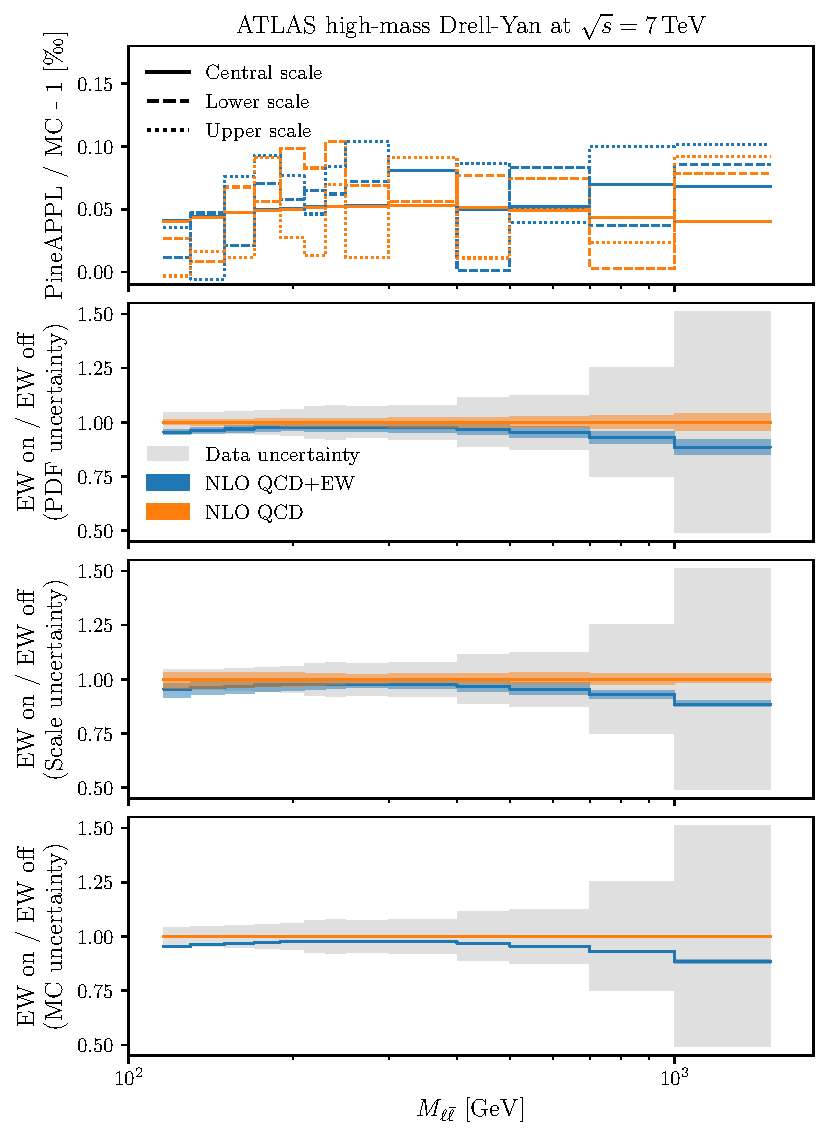
\includegraphics[width=0.5\textwidth]{figures/pineappl_ATLASZHIGHMASS49FB}
    \caption{PineAPPL comparison for ATLAS high-mass Drell--Yan at $\sqrt{s}=7$ TeV.}
    \label{fig:atlaszhighmass49fb}
\end{figure}

\begin{figure}
    \centering
    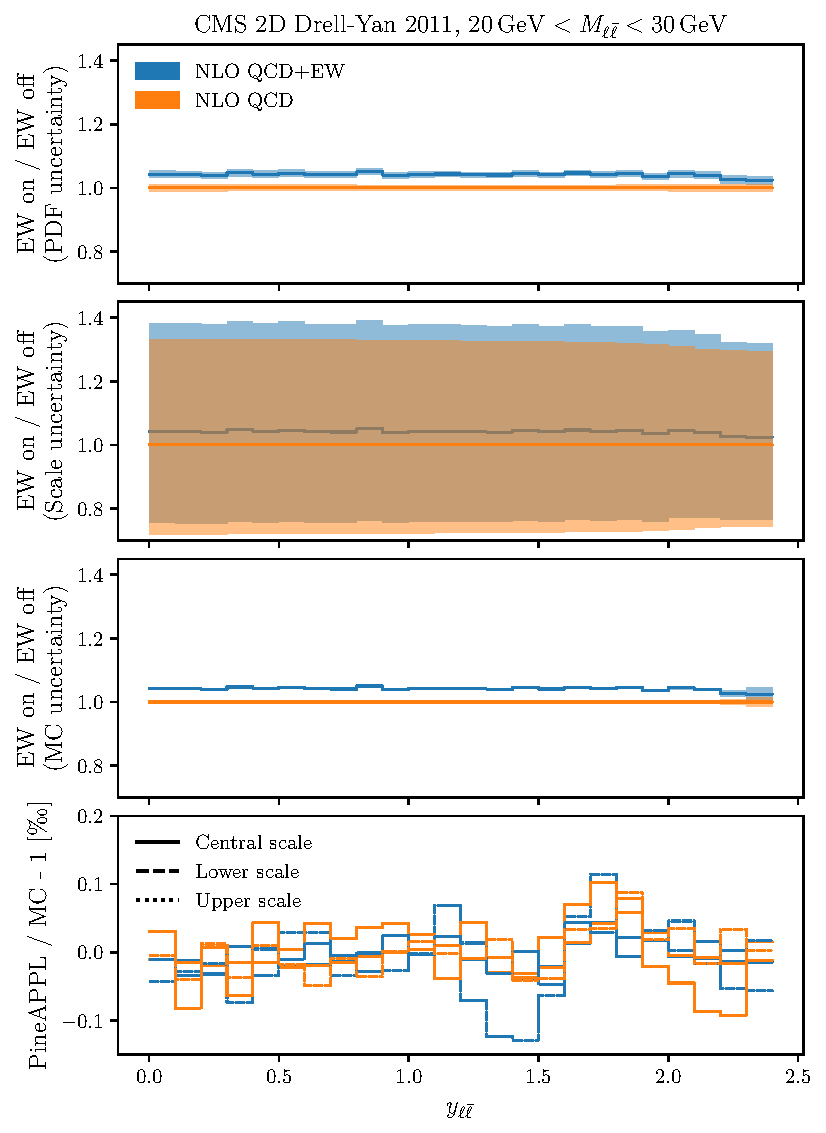
\includegraphics[width=0.5\textwidth]{figures/pineappl_CMSDY2D11_bin1}%
    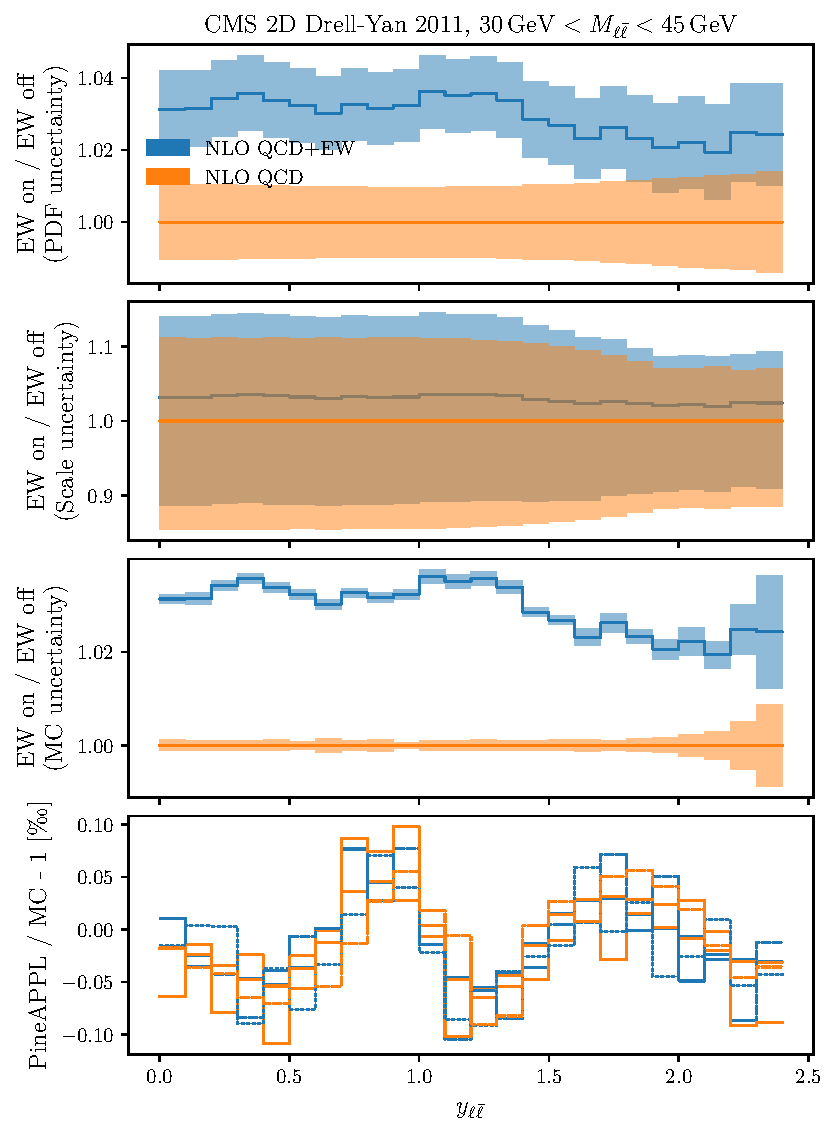
\includegraphics[width=0.5\textwidth]{figures/pineappl_CMSDY2D11_bin2}
    \caption{PineAPPL comparison for CMS 2D Drell--Yan.}
    \label{fig:cmsdy2d11_bins12}
\end{figure}

\begin{figure}
    \centering
    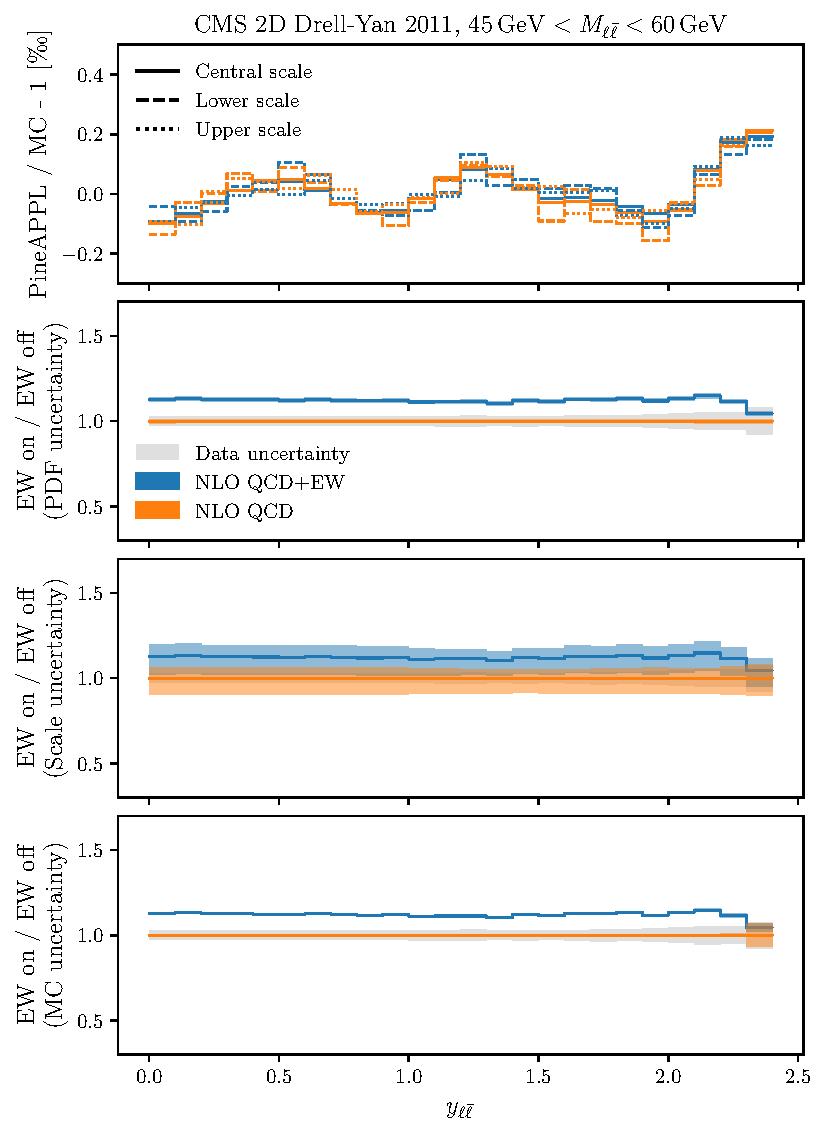
\includegraphics[width=0.5\textwidth]{figures/pineappl_CMSDY2D11_bin3}%
    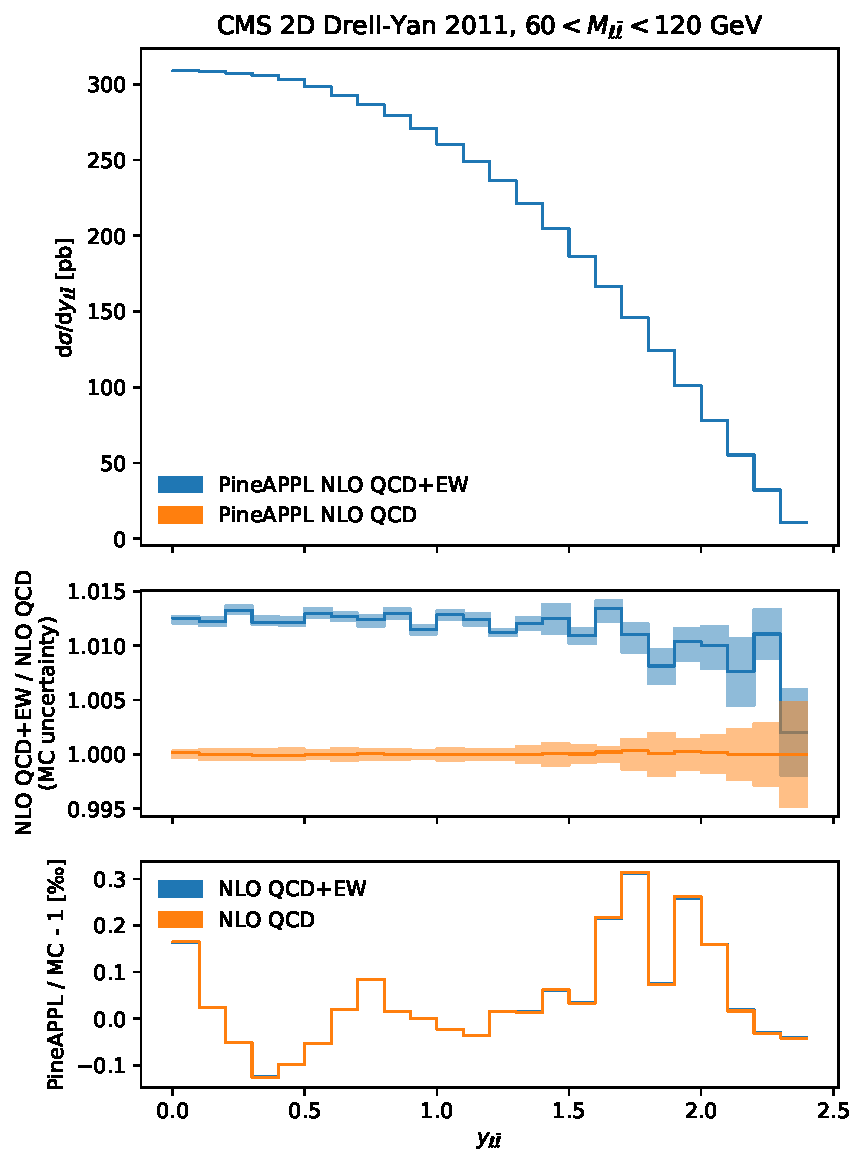
\includegraphics[width=0.5\textwidth]{figures/pineappl_CMSDY2D11_bin4}
    \caption{PineAPPL comparison for CMS 2D Drell--Yan.}
    \label{fig:cmsdy2d11_bins34}
\end{figure}


\begin{figure}
    \centering
    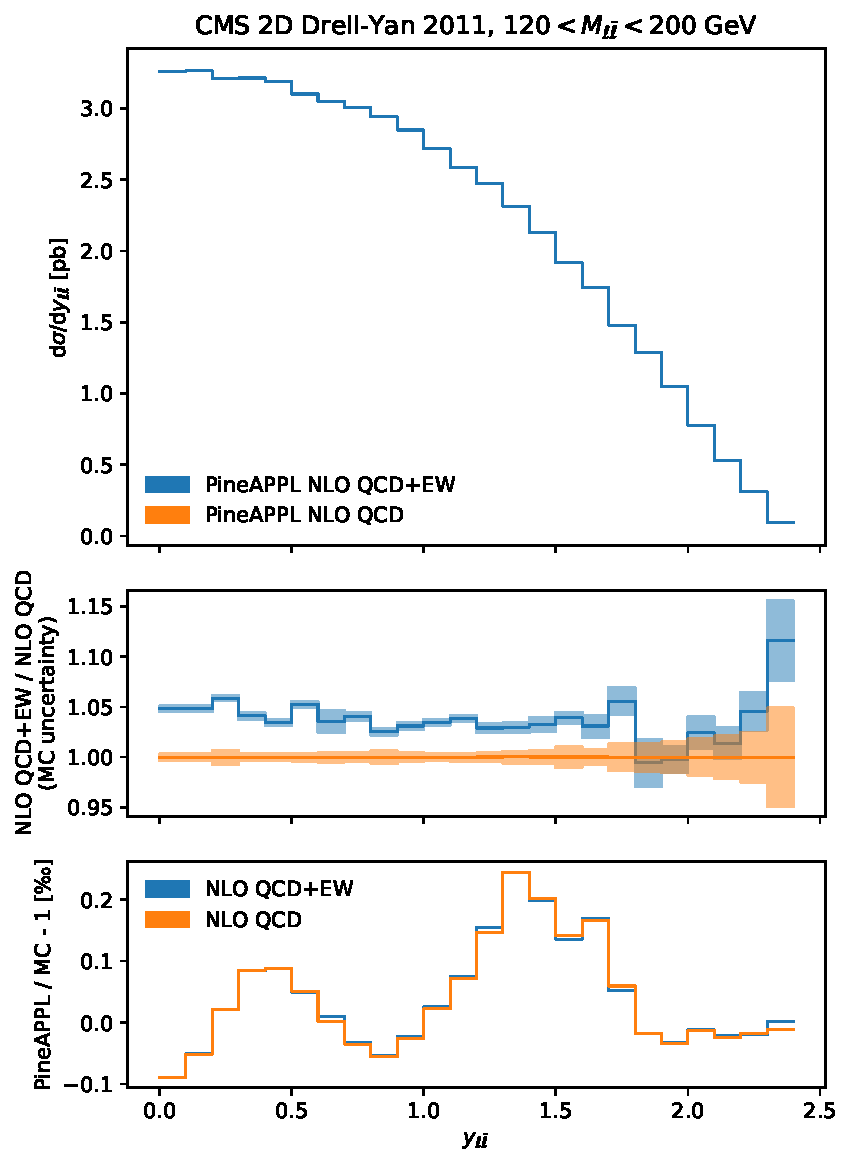
\includegraphics[width=0.5\textwidth]{figures/pineappl_CMSDY2D11_bin5}%
    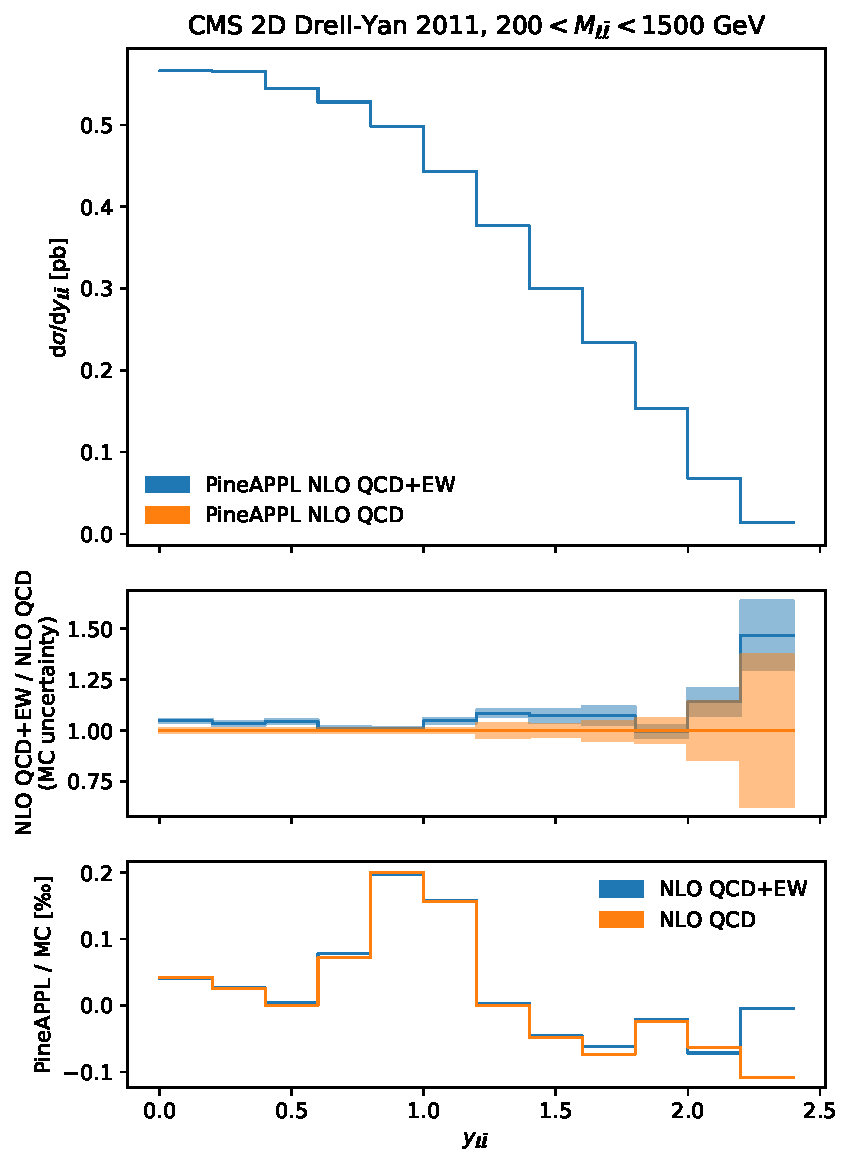
\includegraphics[width=0.5\textwidth]{figures/pineappl_CMSDY2D11_bin6}
    \caption{PineAPPL comparison for CMS 2D Drell--Yan.}
    \label{fig:cmsdy2d11_bins56}
\end{figure}


%ERN 7 Apr: there is consensus on the fact that we should present results for the
%following data sets:
%\begin{itemize}
%\item ATLAS high mass DY distributions, 7 TeV~\cite{Aad:2013iua} (CS);
%\item CMS 2D DY distributions, 7 TeV~\cite{Chatrchyan:2013tia} (CS);
%\item ATLAS top pair differential distributions ($m_{t\bar{t}}$ and $p_T^t$),
%8 TeV~\cite{Aad:2015mbv} (ERN);
%\item CMS $Z$ $pT$ distributions, 13 TeV~\cite{Sirunyan:2019bzr} (ERN).
%\end{itemize}
%
%We agree not to display any LHCb measurement, given that they won't add
%further value to our discussion.
%Note added: we might also want to have a look at the ATLAS 2D and 3D DY
%distributions, 8 TeV~\cite{Aad:2016zzw,Aaboud:2017ffb}, if time allows
%us to do so.
%
%CS 25 Jun: We've agreed to show basically two types of plots: 1) technical plots showing the good agreement between the MC compared to the results from the grids, and 2) phenomenological results showing larger EW corrections, for example.
%In the aMCfast paper both is shown in single plot, but since we have more to show, I suggest the following: for the technical plots we show a 2x2 matrix of plots, each showing the difference of the grid result compared to the MC result, in the following fashion:
%\begin{itemize}
%\item NLO QCD with low statistics,
%\item NLO QCD+EW with low statistics,
%\item NLO QCD with high statistics, and finally
%\item NLO QCD+EW with high statistics,
%\end{itemize}
%each showing a few scale variations.
%These plots then clearly show that no matter what corrections you choose, no matter the statistics, and no matter the scale variation, the agreement is always excellent.
%In any case I would like to avoid showing a plot with absolute numbers and low statistics, which looks a bit ridiculous in my opinion (look at figure 1, left side, top plot of the aMCfast paper).
%
%Finally we can show another series of plots, which in my opinion should be very similar to the usual pheno paper plots: absolute numbers with a scale variation band, maybe a few corrections shown in the same plot and then in the bottom relative corrections.
